\documentclass[../physical_computing.tex]{subfiles}

\begin{document}

\chapter{Logic and Integers}
\label{sec:chapter1_logic_integers}

\section{Logic Gates}
\label{sec:logicgates}

We start our physical computing course where all beginners courses on digital circuits begin, with logic gates.
A logic gate is an abstract operation having a single digital output and one or more digital inputs. There are seven
logic gates that you will see on schematics. The simplest of them is a NOT gate, or inverter, mentioned in the preface,
whose output is $1$ when its single input is $0$, and $0$ when the input is $1$. The next simplest gates each have two inputs. The two input AND gate has output $1$ only when both its inputs are $1$, the two input OR gate has output $1$ when either or both of its inputs are $1$, and the two input XOR (exclusive or) gate has output $1$ when either one, but not both, of its inputs are $1$. That's four so far. The other three gates consist of the AND, OR and XOR gates with an inverter on the output, forming the NAND, NOR and XNOR gates. The six two-input gates generalise to more than two inputs. For example, a 3 input XOR gate has output $1$ when any one, but not more than one, of its inputs is $1$.

An alternative to these written descriptions of functionality is to tabulate the outputs for each possible combination of inputs. Such tables are called truth tables. The truth tables for the four gates NOT, AND, OR and XOR are shown in Figure \ref{fig:logic_gates_figure}
along with the symbols representing the gates. The figure caption tells you how to draw the other three gates NAND, NOR and XNOR. 

\begin{figure}[t]
\centering
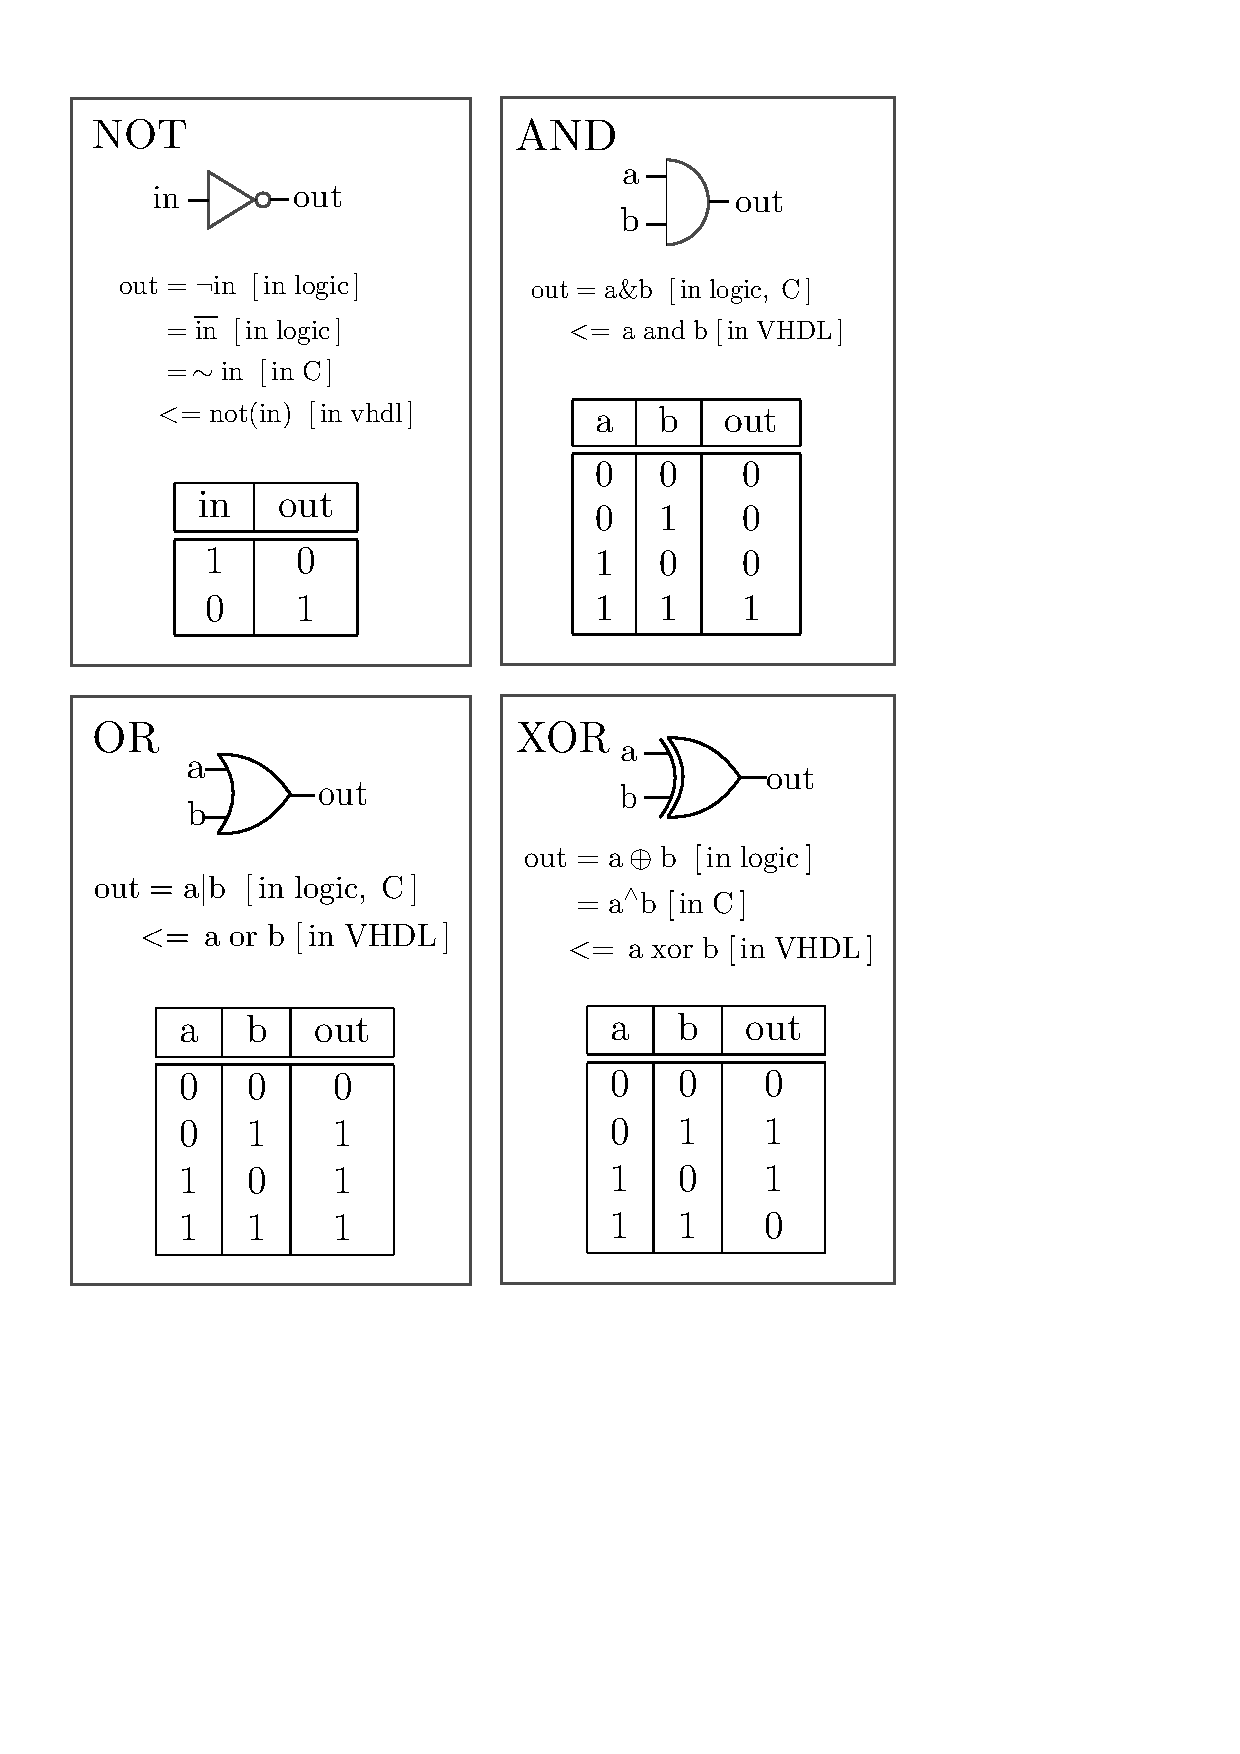
\includegraphics[width=0.5\textwidth]{figures/logic_gates_figure.pdf}
\caption{\label{fig:logic_gates_figure} Truth tables and symbols for four of the seven logic gates commonly encountered. The other three, NAND, NOR and XNOR are obtained by adding a not at the output of AND, OR and XOR, respectively. The symbols are the same as for AND, OR and XOR except for the addition of a small circle like that on the right side of the NOT gate. Sometimes you will also see a small circle on one of the input leads before the gate body. For example, if this circle before the body of the AND gate appears on the b input, it means `a and not b.'}
\end{figure}

\section{De Morgan's Laws}
\label{sec:demorgan}

It turns out that you can build AND gates out of OR gates and NOT gates, or OR gates out of AND gates and NOT gates, as a consequence of a useful piece of maths that comes from the theory of sets, called De Morgan's laws. In the theory of sets, if $A$ and $B$ are each sets, then $A\cap B$ is called the intersection of $A$ and $B$, and means all the elements that are in both set A and set B, and $A\cup B$ is called the union of $A$ and $B$ and means all the elements that are set A or set B. So there is a direct correspondence between the logical $\rm AND$ and the intersection, and between the logical $\rm OR$ and the union. What about $\rm NOT$? In set theory the symbol for all the elements not in set $A$ is the complement of $A$, or $\overline{A}$. There are two De Morgan's Laws, and both can be stated either in set notation or in logic notation. The logical statements are

\begin{figure}[h!]
    \centering
    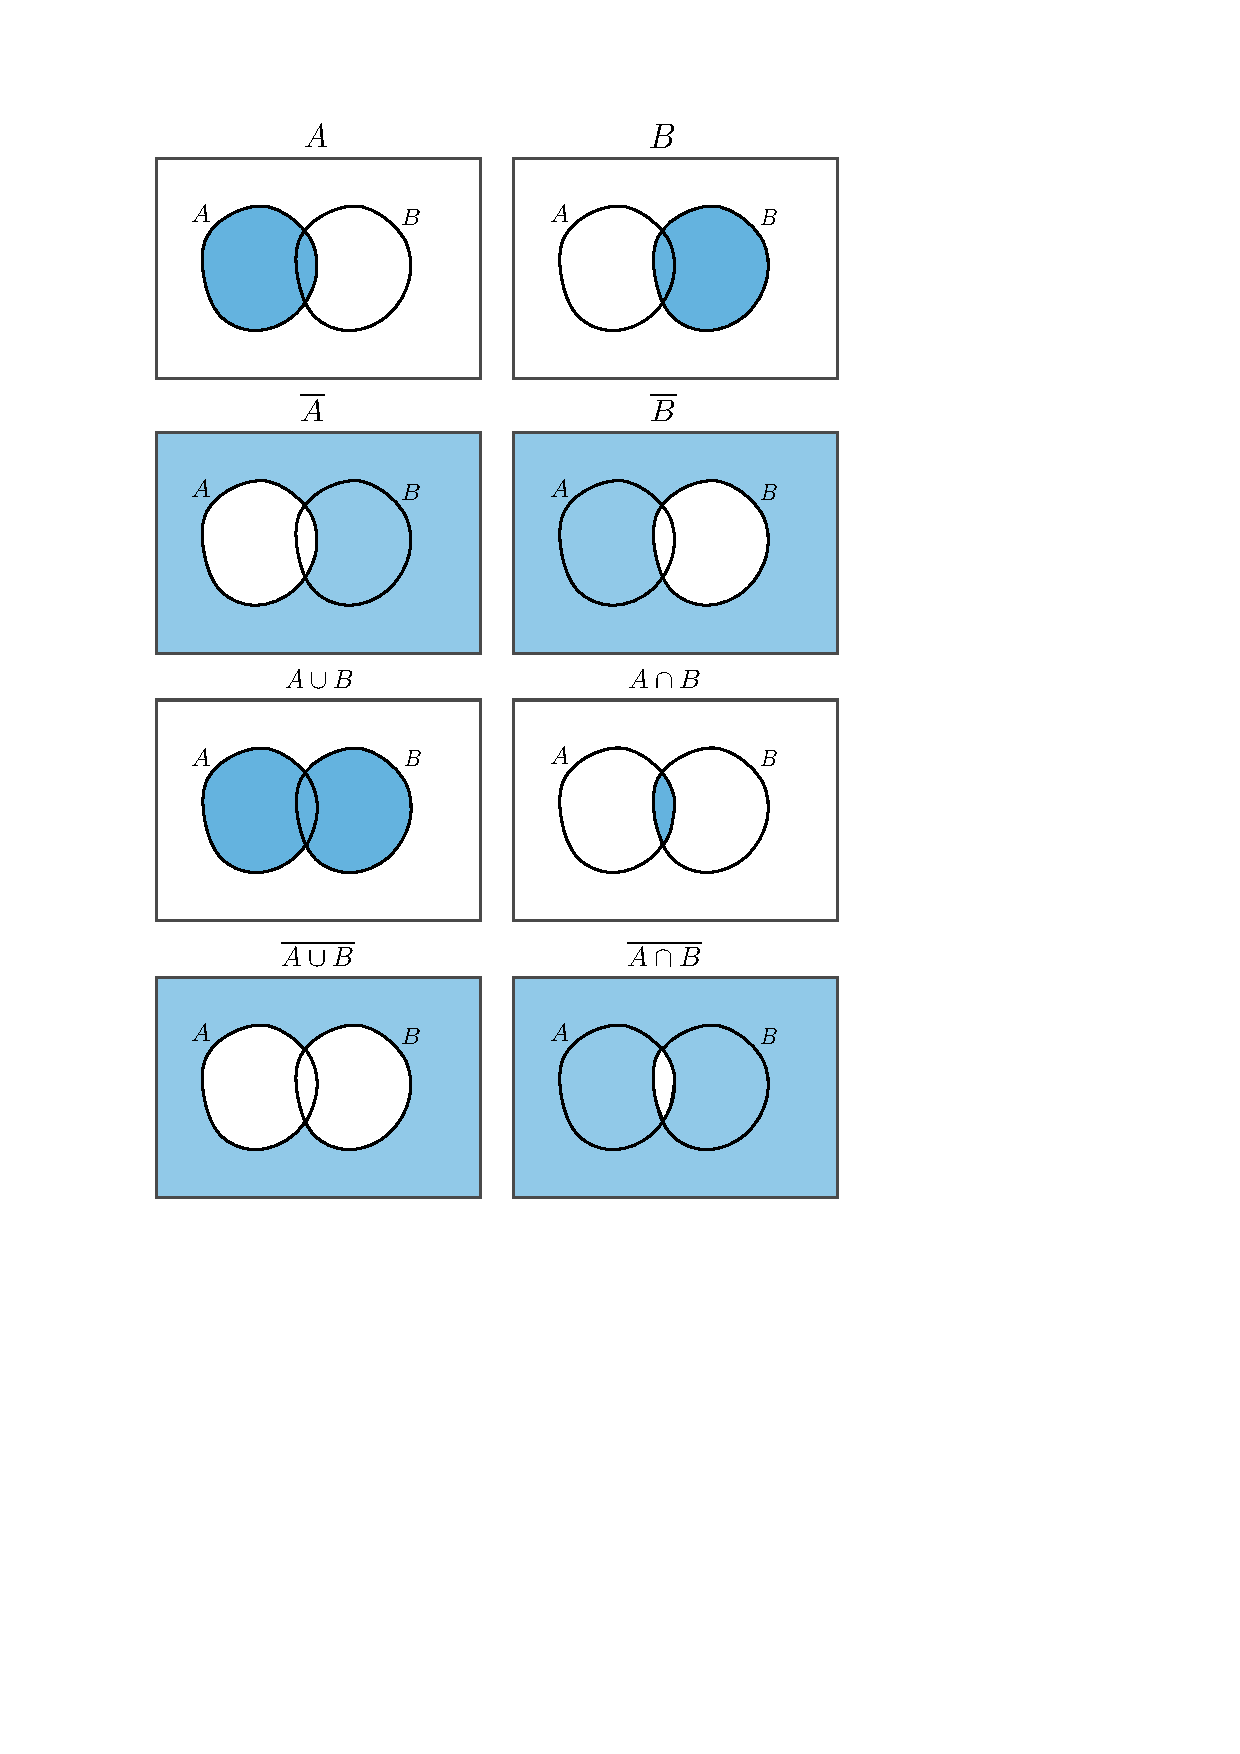
\includegraphics[width=0.45\textwidth]{figures/venn_diagram_figure.pdf}
    \caption{\label{fig:venn_diagram_figure} Venn diagrams illustrating De Morgan's laws.}
\end{figure}

\begin{align}
\neg(a\&b) &= \neg a | \neg b
\label{eq:demorganone} \\
\neg(a|b)&=\neg a \& \neg b.
\label{eq:demorgantwo} \\
\nonumber
\end{align}
In words, Equation \ref{eq:demorganone} states that not(a and b) is the same as (not a) or (not b), and Equation \ref{eq:demorgantwo} states that not(a or b) is the same thing as (not a) and (not b). The same two laws can be stated in set notation as
\begin{align}
    \overline{A\cap B}&=\overline{A}\cup\overline{B}
    \label{eq:demorganoneset} \\
    \overline{A\cup B}&=\overline{A}\cap\overline{B}.
    \label{eq:demorgantwoset} \\ \nonumber
\end{align}
If you like Venn diagrams, you can prove De Morgan's Laws with them. This is done in Figure \ref{fig:venn_diagram_figure}. The rectangle represents all objects in some space, everything inside the left hand ellipse is in set A, and everything inside the right hand ellipse is in set B. The complements of $A$ and $B$ are shown in the second row. The union and intersection of $A$ and $B$ are in the third row. The fourth row shows the complements of the union and the intersection of $A$ and $B$. The union of $\overline{A}$ and $\overline{B}$ is the areas that are blue in either of the diagrams in the second row. This is everything except the thin white sliver common between both $A$ and $B$, in other words it is the complement of the intersection of $A$ and $B$. This proves De Morgan's first law, Equations \ref{eq:demorganone} and \ref{eq:demorganoneset}. The intersection of $\overline{A}$ and $\overline{B}$ is the areas that are blue in both of the diagrams in the second row. This is everything that isn't in either of the white ellipses of $A$ or $B$, in other words it is the complement of the union of $A$ and $B$. This proves De Morgan's second law, Equations \ref{eq:demorgantwo} and \ref{eq:demorgantwoset}.

De Morgan's laws simplify the job of chip designers since essentially all of the logic gate elements on a chip may be fabricated out of either OR gates or AND gates, plus inverters. Figure \ref{fig:de_morgan_logic} is a third statement of De Morgan's laws in terms of the symbols for the gates themselves.

\begin{figure}[htbp]
    \centering
    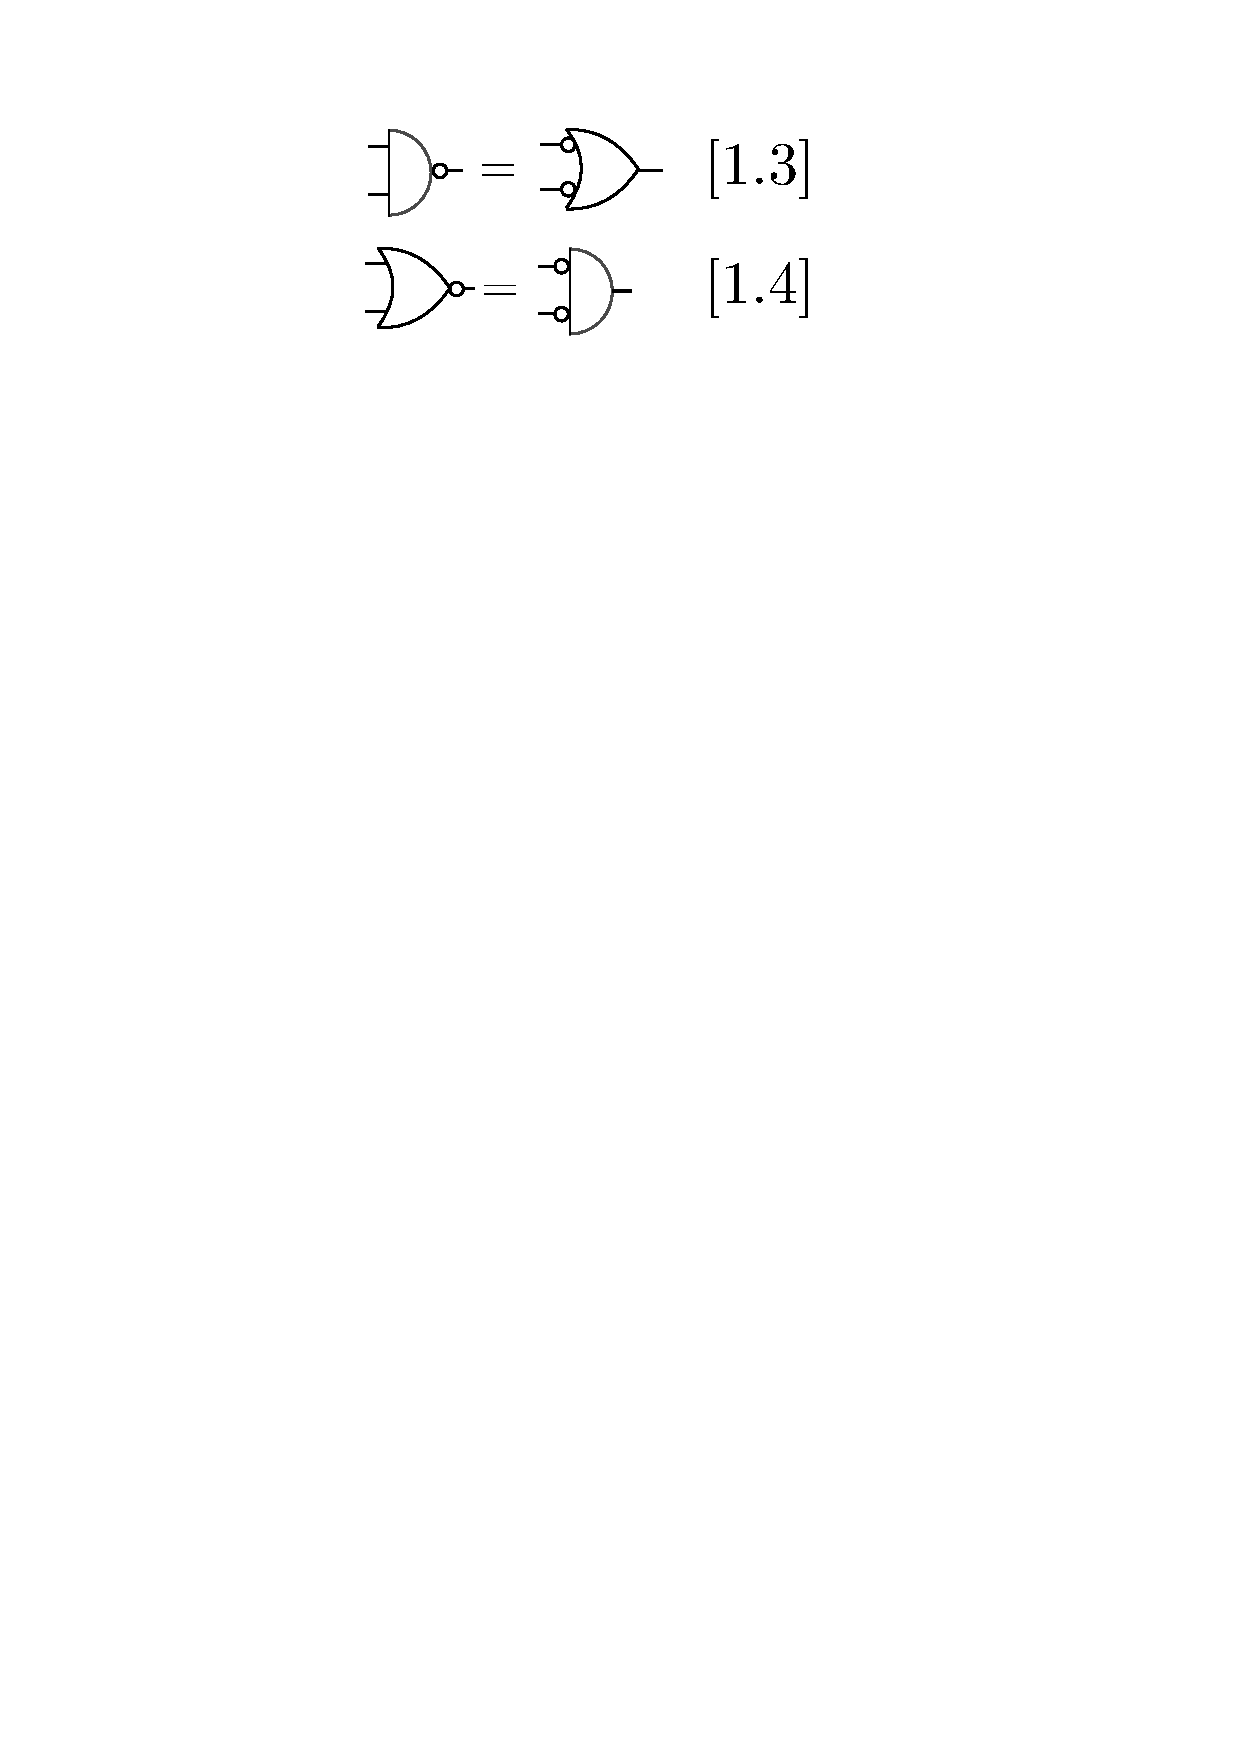
\includegraphics[width=0.2\textwidth]{figures/de_morgan_logic.pdf}
    \caption{\label{fig:de_morgan_logic} De Morgan's laws in terms of the equivalence between different types of logic gate.}
\end{figure}

\section{Parallel Buses}
\label{sec:parallel_buses}

We aren't going to get very far if we only ever deal with one bit at a time. The simplest way to streamline manipulations of multiple bits is to perform the same operation on many bits in parallel. A collection of bits in parallel is called a bus, and the number of bits in the bus is called the bus width. Frequently buses consist of 8, 16 or 32 bits in parallel. There are other kinds of buses other than parallel, and we will discuss some of these presently, but for now just imagine an assembly of signals in a set of wires. Buses are ordered. In other words, the position of a particular bit of a bus is well defined. Usually we think of a bus as an ordered set of bits from left to right, with the rightmost bit called the least significant bit, or LSB, and the leftmost bit called the most significant bit, or MSB. This is in preparation for use of parallel buses to represent integers, which we will discuss in Section \ref{sec:logic_and_integers}. 

The logic operations defined in Section \ref{sec:logicgates} were so far discussed as operating on a single bit, but they can also operate on buses containing many bits, so long as each input and output has the same bus width. Used in this way, the logic operations NOT ($\neg$), AND ($\&$), OR ($|$), XOR ($\oplus)$, NAND ($\neg\&$), NOR ($\neg|$) and XNOR ($\neg\oplus$) are examples of `bitwise' operations, in that they operate on each bit separately and do the same thing to all the bits. So, for example,
\begin{align}
    \neg\,B00010000&=B11101111
    \label{eq:first_bus_operation}
\end{align}
 and
\begin{align}
   B10101010\,|\,B00010000\,&=\,B10111010.
   \label{eq:second_bus_operation}
\end{align}
 Here I have used the notation of a leading $B$ to mean that the sequence of digits following represents a bus of bits - just a way of expressing whether the bits in a bus are high or low, $1$ or $0$, or equivalently true or false.
 
 There are other binary operations that can only meaningfully act on parallel buses of bits. Bit shifting operations, in particular, involve shifting the values in all the bits in a bus to the left (in the direction of the most significant bit) or to the right (in the direction of the least significant bit). As a consequence, either the rightmost or the leftmost bit falls off the end of the bus and is lost, and a gap appears at the other end. In a logical bit-shift operation, the gap is filled with a zero. In an arithmetic bit shift, the gap is filled with a copy of the value in the bit that must moved along to create the gap. Finally, you could possibly place the value in the bit that fell off the other end of the bus in this position. All three types of bitshift operations can sometimes be needed. Where the bus is representing logical rather than arithmetical data, logical bit shifting is the most common. An exercise in Appendix \ref{sec:logic_in_vhdl} will show you how to execute logical bit shifts on buses representing logical data in the hardware description language VHDL.
 
 The use of binary operations to simplify and speed up computer code is an interesting subject. There is a nice book by Warren \cite{Warren:10.5555/2462741} where you can read about logical consequences of De Morgan's laws and mathematical tricks involving bitwise logic operations combined with bit shifts, particularly in Chapters 1 and 2, which I will make available to you on Collaborate.

\section{Logic and Integer Arithmetic}
\label{sec:logic_and_integers}

\subsection{Logic and the Foundations of Mathematics}
\label{sec:logicandmathsfoundations}

De Morgan's laws are an example of the connection between the theory of sets and logic. This is natural because both sets and logic are closely connected to the foundations of mathematics. The drive to build a logical foundation for mathematics was an area of intense activity at the turn of the 20th century. The famous series of books, Principia Mathematica, by Russell and Whitehead \cite{Whitehead:268025}, an attempt to build a consistent and complete logical foundation for mathematics, famously collided with the philosophy of Kurt G\"odel who proved that the task is impossible. Modern formulations of axiomatic set theory, or the logical foundations of mathematics, are based on Zermelo-Fraenkel set theory, and it is in this context that modern developments in the logical foundation of mathematics are usually discussed. The subject of the logical foundations of mathematics is fascinating. If you are interested, and there are many popular books on the subject which will stretch your mind, especially if you try and do the puzzles \cite{Hofstadter:99665,Smullyan} !

Fortunately we do not need to construct a complete logical basis for mathematics, only to work out some ways of using logic gates to do simple arithmetic, which is much easier. Nonetheless, we shall quickly discover that in using logic to do mathematics you have to be careful to avoid encountering difficulties. These difficulties shall be discussed in Chapter \ref{sec:registers}.

\subsection{Binary Representation of Positive Integers}
\label{sec:postiveintegers}

Let us first consider representation of integers. Bits naturally lead to the use of binary numbers to represent integers. Any sensible representation will have the integer zero represented by any number of $0$s, and the integer one represented by a single $1$. If the integers are all positive or zero, then all we need is ordinary binary numbers, so the numbers 0 to 15 can be represented by three binary digits. In ascending order, $B0000$, $B0001$, $B0010$, $B0011$ $B0100$, $B0101$, $B0110$, $B0111$, $B1000$, $B1000$, $B1001$, $B1010$, $B1011$ $B1100$, $B1101$, $B1110$, $B1111$. If we want to represent any larger number than 15, we will need more bits in our binary representation than four. The largest unsigned integer representable using an $N$ bit parallel bus is $2^N-1$.

\subsection{Hexadecimal Notation}
\label{sec:hexadecimal}

I am already getting tired of writing all those zeros and ones, and in digital signal processing it is common to represent collections of binary numbers using hexadecimal, or base 16. Because people commonly have ten figures, we have developed naturallly to have symbols for each of the counting numbers between 0 and 9, and think of larger numbers as groups of 10, or groups of 100, and so on. However, suppose we had actually had 16 fingers! We would then have naturally developed separate symbols for the first 16 integers 0 to 15 that are also each representable by four binary bits. Table \ref{tab:hexadecimal} shows the first 16 numbers from the set of positive integers and zero, together with their decimal and hexadecimal representations.

\begin{table}[hbt]
    \centering
    \begin{tabular}{|c|c|c|}
    \hline
         decimal & binary & hexadecimal \\
         \hline\hline
         0 & B0000 & 0x0 \\
         1 & B0001 & 0x1 \\
         2 & B0010 & 0x2 \\
         3 & B0011 & 0x3 \\
         4 & B0100 & 0x4 \\
         5 & B0101 & 0x5 \\
         6 & B0110 & 0x6 \\
         7 & B0111 & 0x7 \\
         8 & B1000 & 0x8 \\
         9 & B1001 & 0x9 \\
         10 & B1010 & 0xa \\
         11 & B1011 & 0xb \\
         12 & B1100 & 0xc \\
         13 & B1101 & 0xd \\
         14 & B1110 & 0xe \\
         15 & B1111 & 0xf \\
        \hline
    \end{tabular}
    \caption{Decimal, binary and hexadecimal representation of zero and the first fifteen positive integers.}
    \label{tab:hexadecimal}
\end{table}

The hexadecimal notation is extensible to numbers represented by many more bits. For example, on computers integers are commonly represented as 32 bit binary numbers, so that the unsigned integer 1 would be represented as $\rm B00000000000000000000000000000001$. In hexadecimal this is $\rm 0x00000001$, which is still a lot of leading zeros, but you can see how the reduction in the number of symbols by a factor of four when using hexadecimal notation instead of binary is attractive.

\subsection{Binary Counters and Oscillators}
\label{sec:oscillators}

While we are looking at this table, it makes obvious another useful feature of binary numbers, and that is the behaviour of the binary digits. Scan down the column of binary numbers and look only at the least significant bit (LSB). Notice that as the count proceeds, the least significant bit oscillates back and forth between $0$ and $1$ with a period of two counting numbers. Now look at the second-least significant bit. This bit also oscillates back and forth between zero and one, but the period of this oscillation is four counts. The third least significant bit also oscillates periodically with a period of 8 counts, and the most significant bit (MSB) has a period of the full 16 counts. This means that if we can cause a bus to count upwards from zero, each subsequent bit can serve as an oscillator with a period of twice that of the previous bit. It turns out to be very useful indeed to be able to make oscillators with different periods in digital devices, and we shall see the power of this in Chapter \ref{sec:registers}.

\subsection{Overflows in Binary Arithmetic}
\label{sec:overflows}

We have already realised that we need more than four bits to represent a positive binary number greater than 15. What is the convention for dealing with overflows? What happens when you add 1 to 0xf ? We will operate with the following convention, following digital signal processing conventions: {\it overflows are disregarded}. If you require more bits than you have designed into your system to get the right answer, it's just tough - you should have used more bits. While this might sound harsh, in fact the convention that overflows are ignored is very useful indeed.

The first reason for this is to do with counters. As alluded to before, if we count up in binary, each successively more significant bit behaves like an oscillator with half the period of the bit to the right. What about the most significant bit? What does it do? It starts out as 0, then half way to the maximum capacity of the bus, it switches to 1. What happens when it reaches full capacity? This is when all the bits are $1$. The next number in the sequence, {\it ignoring the overflow} is all zeros. In other words, the counter just resets to zero, and then keeps counting. A counter that starts at zero, then gets to the maximum number that can be represented with the number of bits, then resets to zero automatically and starts again, is very useful indeed!

There's another very useful application of ignoring overflows. It means that a binary number of N bits containing all 1s is adjacent in the sequence of binary numbers to a binary number containing all 0s. This comes in very handy when representing negative integers with a system called {\it twos complement} which we will discuss in the next section.

To summarise this section, in a binary representation of numbers, overflows are ignored. If you have 4 bits, then all numbers are represented using 4 bits, and if you end up running off the end, you neglect any overflows and instead your sequence wraps around back to the other end.

\subsection{Negative Integers}
\label{sec:negatives}

What about if we have negative integers? These are almost always represented using a method called twos complement. Suppose we have 4 bits in our binary representation. So far we have thought of these as representing the unsigned integers between 0 and 15. However, recall that the binary number $B1111$, neglecting overflows, is adjacent to the binary number $B0000$. How about using $B1111$ to represent -1? Following the same logic, $B1110$ is adjacent to $B1111$, so it must be -2. Carrying on with this argument, we reach a binary four-bit twos complement representation for the signed integers in the range $[-8,+7]$,

\begin{table}[hbt]
    \centering
    \begin{tabular}{|c|c|c|}
    \hline
         decimal & binary & hexadecimal \\
         \hline\hline
         0 & B0000 & 0x0 \\
         1 & B0001 & 0x1 \\
         2 & B0010 & 0x2 \\
         3 & B0011 & 0x3 \\
         4 & B0100 & 0x4 \\
         5 & B0101 & 0x5 \\
         6 & B0110 & 0x6 \\
         7 & B0111 & 0x7 \\
         -8 & B1000 & 0x8 \\
         -7 & B1001 & 0x9 \\
         -6 & B1010 & 0xa \\
         -5 & B1011 & 0xb \\
         -4 & B1100 & 0xc \\
         -3 & B1101 & 0xd \\
         -2 & B1110 & 0xe \\
         -1 & B1111 & 0xf \\
        \hline
    \end{tabular}
    \caption{Decimal, binary and hexadecimal symbols for the twos complement representation of the signed integers in the range $-8$ to $+7$ inclusive.}
    \label{tab:twoscomplement}
\end{table}

You might notice that moving from $-1$ to $-8$ is a binary count upwards but with the symbols $1$ and $0$ reversed. This means that there is a simple logical way to deduce the binary representation of $-x$ from the binary representation of $+x$. This is
\begin{align}
    -x=\neg x+1.
\end{align}
Let us check that this works. For example, the binary representation of 3 is $B0011$. We take the bitwise not of this binary sequence to get $B1100$, then we add one to this to get $B1101$. From Table \ref{tab:twoscomplement} this represent -3. Try a couple of others. Note that it won't work for -8, because +8 cannot be represented in twos complement signed integer arithmetic using only four bits.

\subsection{Integer addition and multiplication}
\label{sec:addmultiply}

I am about to teach you how to add and multiply binary numbers by hand as you might have learned to do in school for decimal numbers. Of course, there are calculators that have a binary mode - indeed, yours probably does. You can do your binary calculations there, or check your manual calculations using them. There are also online binary and hexadecimal calculators - see, for example \url{calculator.net/binary-calculator.html}.

When you were at school you were probably taught about column addition as a way of adding together two numbers each of which had multiple non-zero digits. You basically write out the two numbers one above the other with each succesive digit aligning vertically with the other number to be added. You then add the digits in the corresponding columns starting with the least significant digit and moving across until you have done the most significant one. The interesting case is when the sum of the two digits exceeds the capacity of the symbols available from a single digit. In this case you 'carry' the difference to the next column, usually writing the carried number below the output to remind you to add it on when you get to the next column. If there are any carry digits left at the end, these are added on the left. 

It's almost the same thinking about binary addition, except the 'columns' instead of being $1$, $10$, $100$ etc are $1$, $2$, $4$, $\cdots$. In both cases, the M\textsuperscript{th} column represents $\rm (base)^{(M-1)}$. The only other modification is that you methodically {\it ignore the overflows}. Let us do some examples. For a start, $2+3$ or $B0010+B0011$. Figure \ref{fig:addition_example_1} shows how this is carried out using column addition.
\begin{figure}[h!]
    \centering
    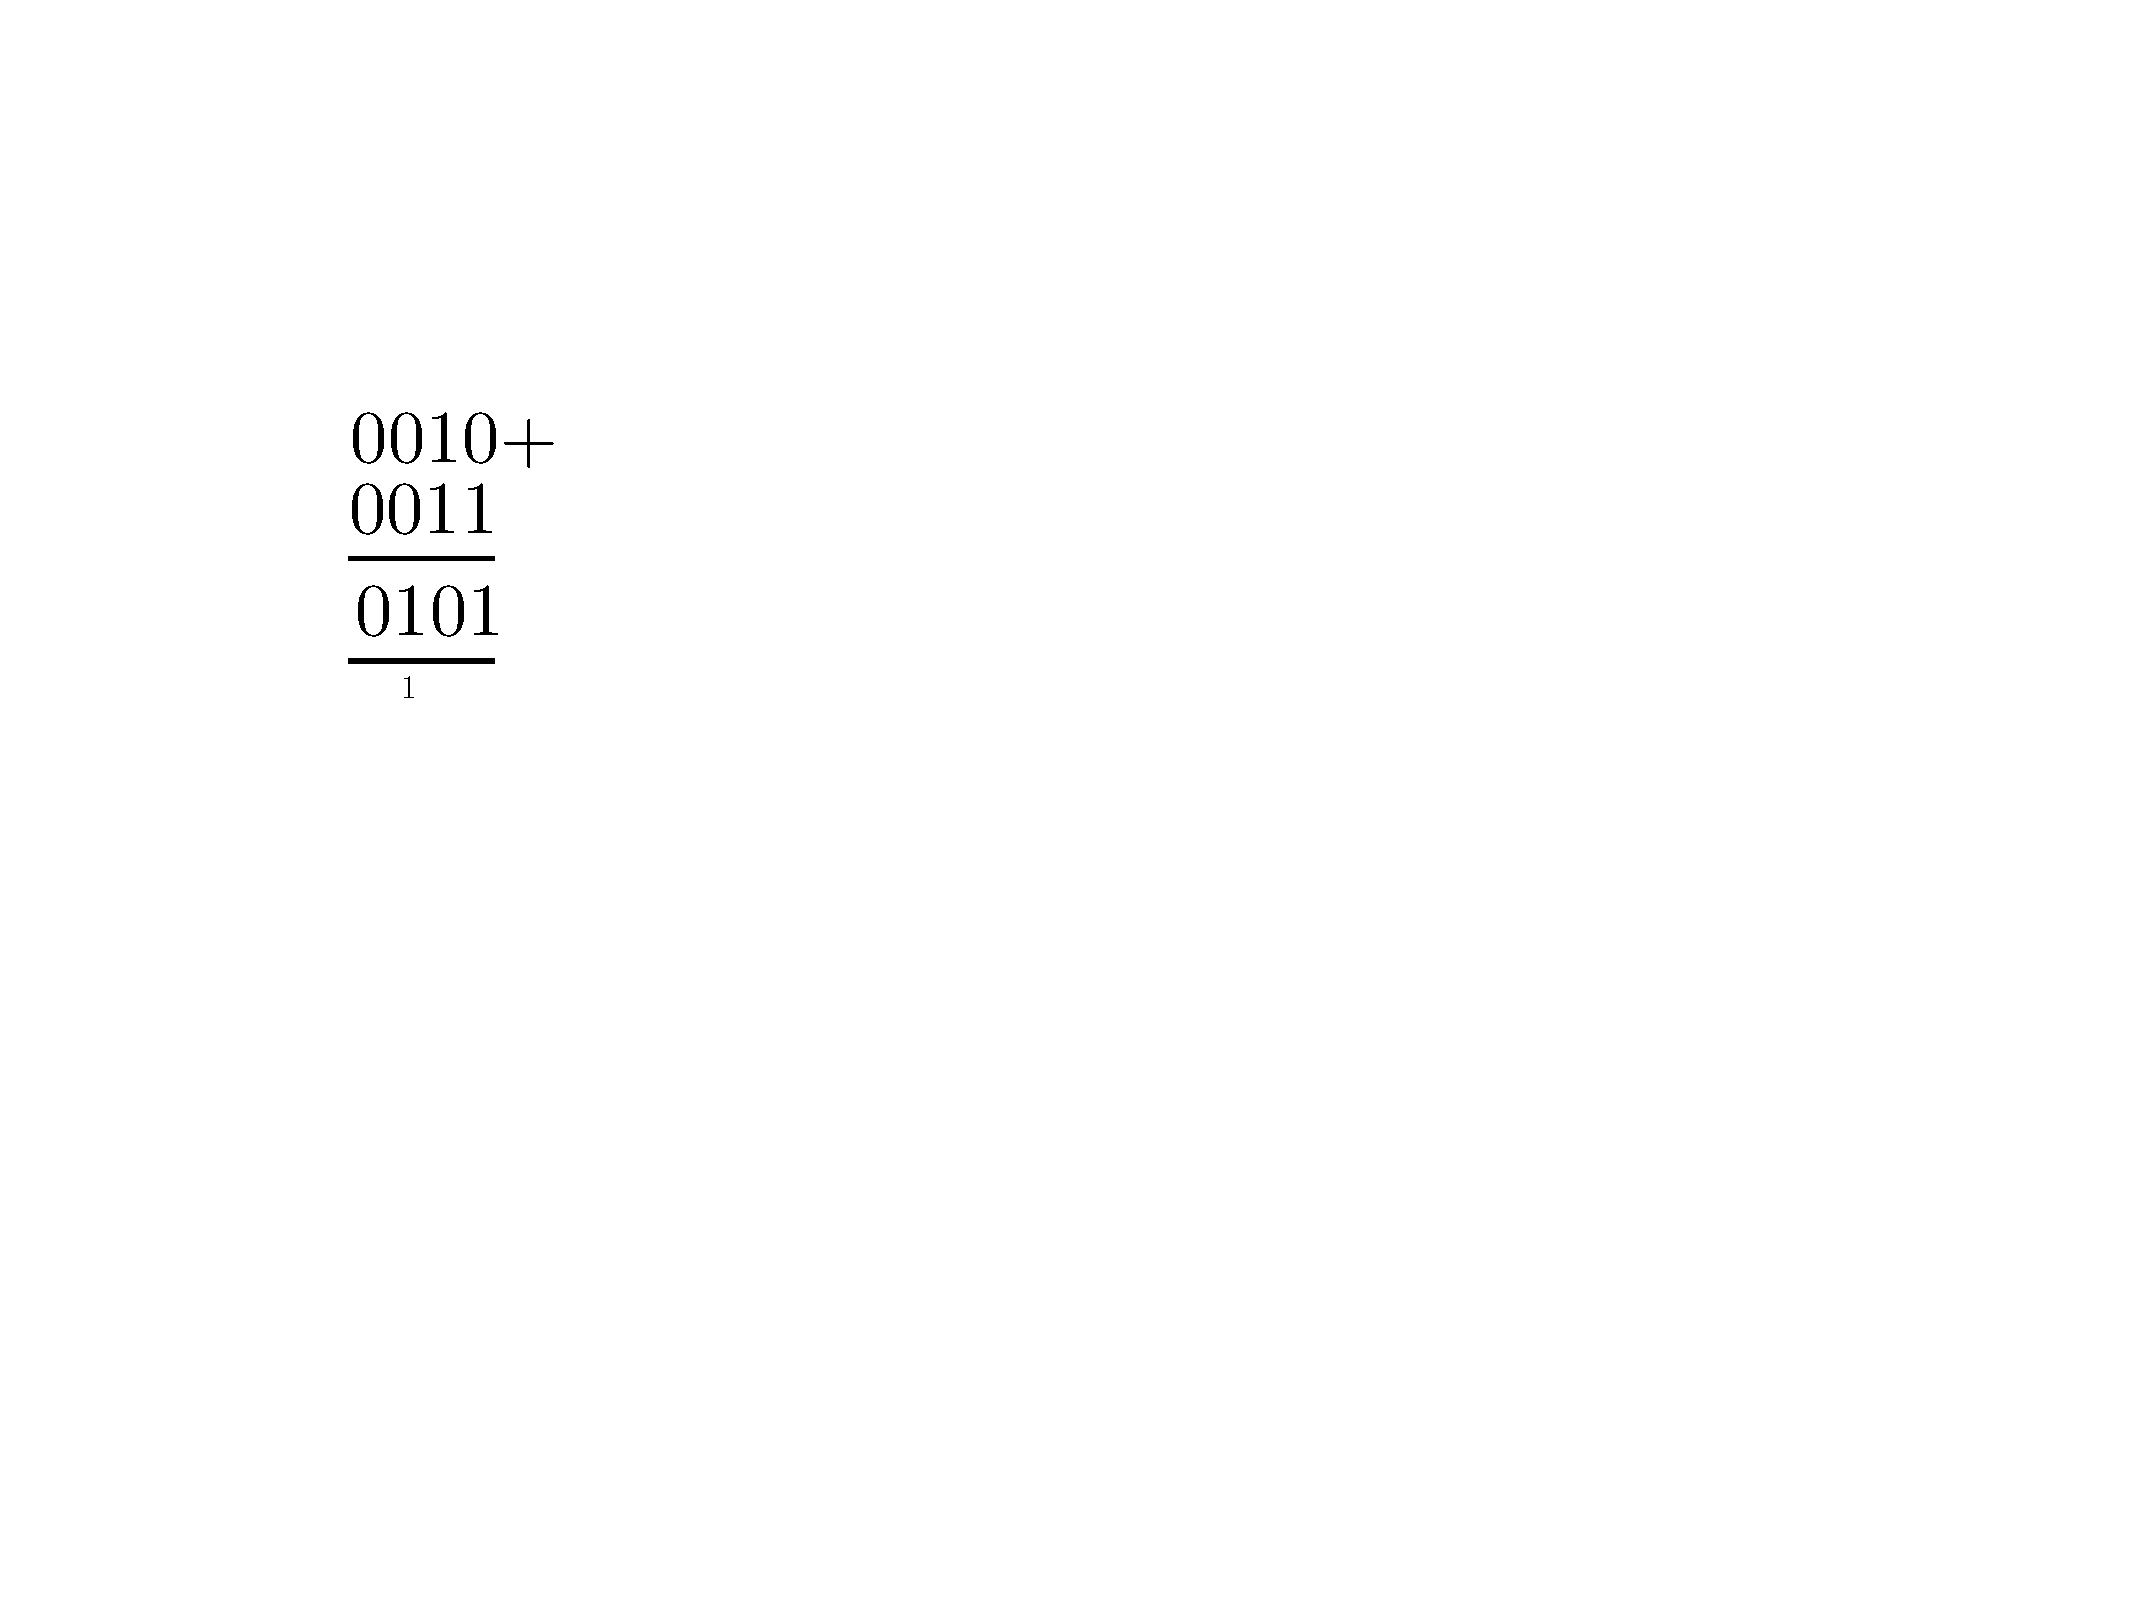
\includegraphics[width=0.1\textwidth]{figures/addition_example_1.pdf}
    \caption{Adding 2 and 3 in binary.}
    \label{fig:addition_example_1}
\end{figure}
In this example, the second column addition results in a carry of $B1$ to the third column, and the third column then just contains that $B1$, so that the overall answer is $1$ times $2^2$ + $1$ times $2^0$, or five.

In the next example, shown in Figure \ref{fig:addition_example_2}, we carry out $-3+7$. The four bit binary representation of $+7$ is $B0111$. To obtain the binary representation of $-3$ we start with $+3$ which is $B0011$. We first do a bitwise not, leading to $B1100$, then we add a least significant bit, $B0001$, to obtain $B1101$, and that's our four-bit binary representation of $-3$. Finally, we carry out the column addition. Notice that when we get the answer we truncate at 4 bits, discarding the overflow $1$. This leads to the correct binary representation of the answer, $B0100$, which is +4.
\begin{figure}[h!]
    \centering
    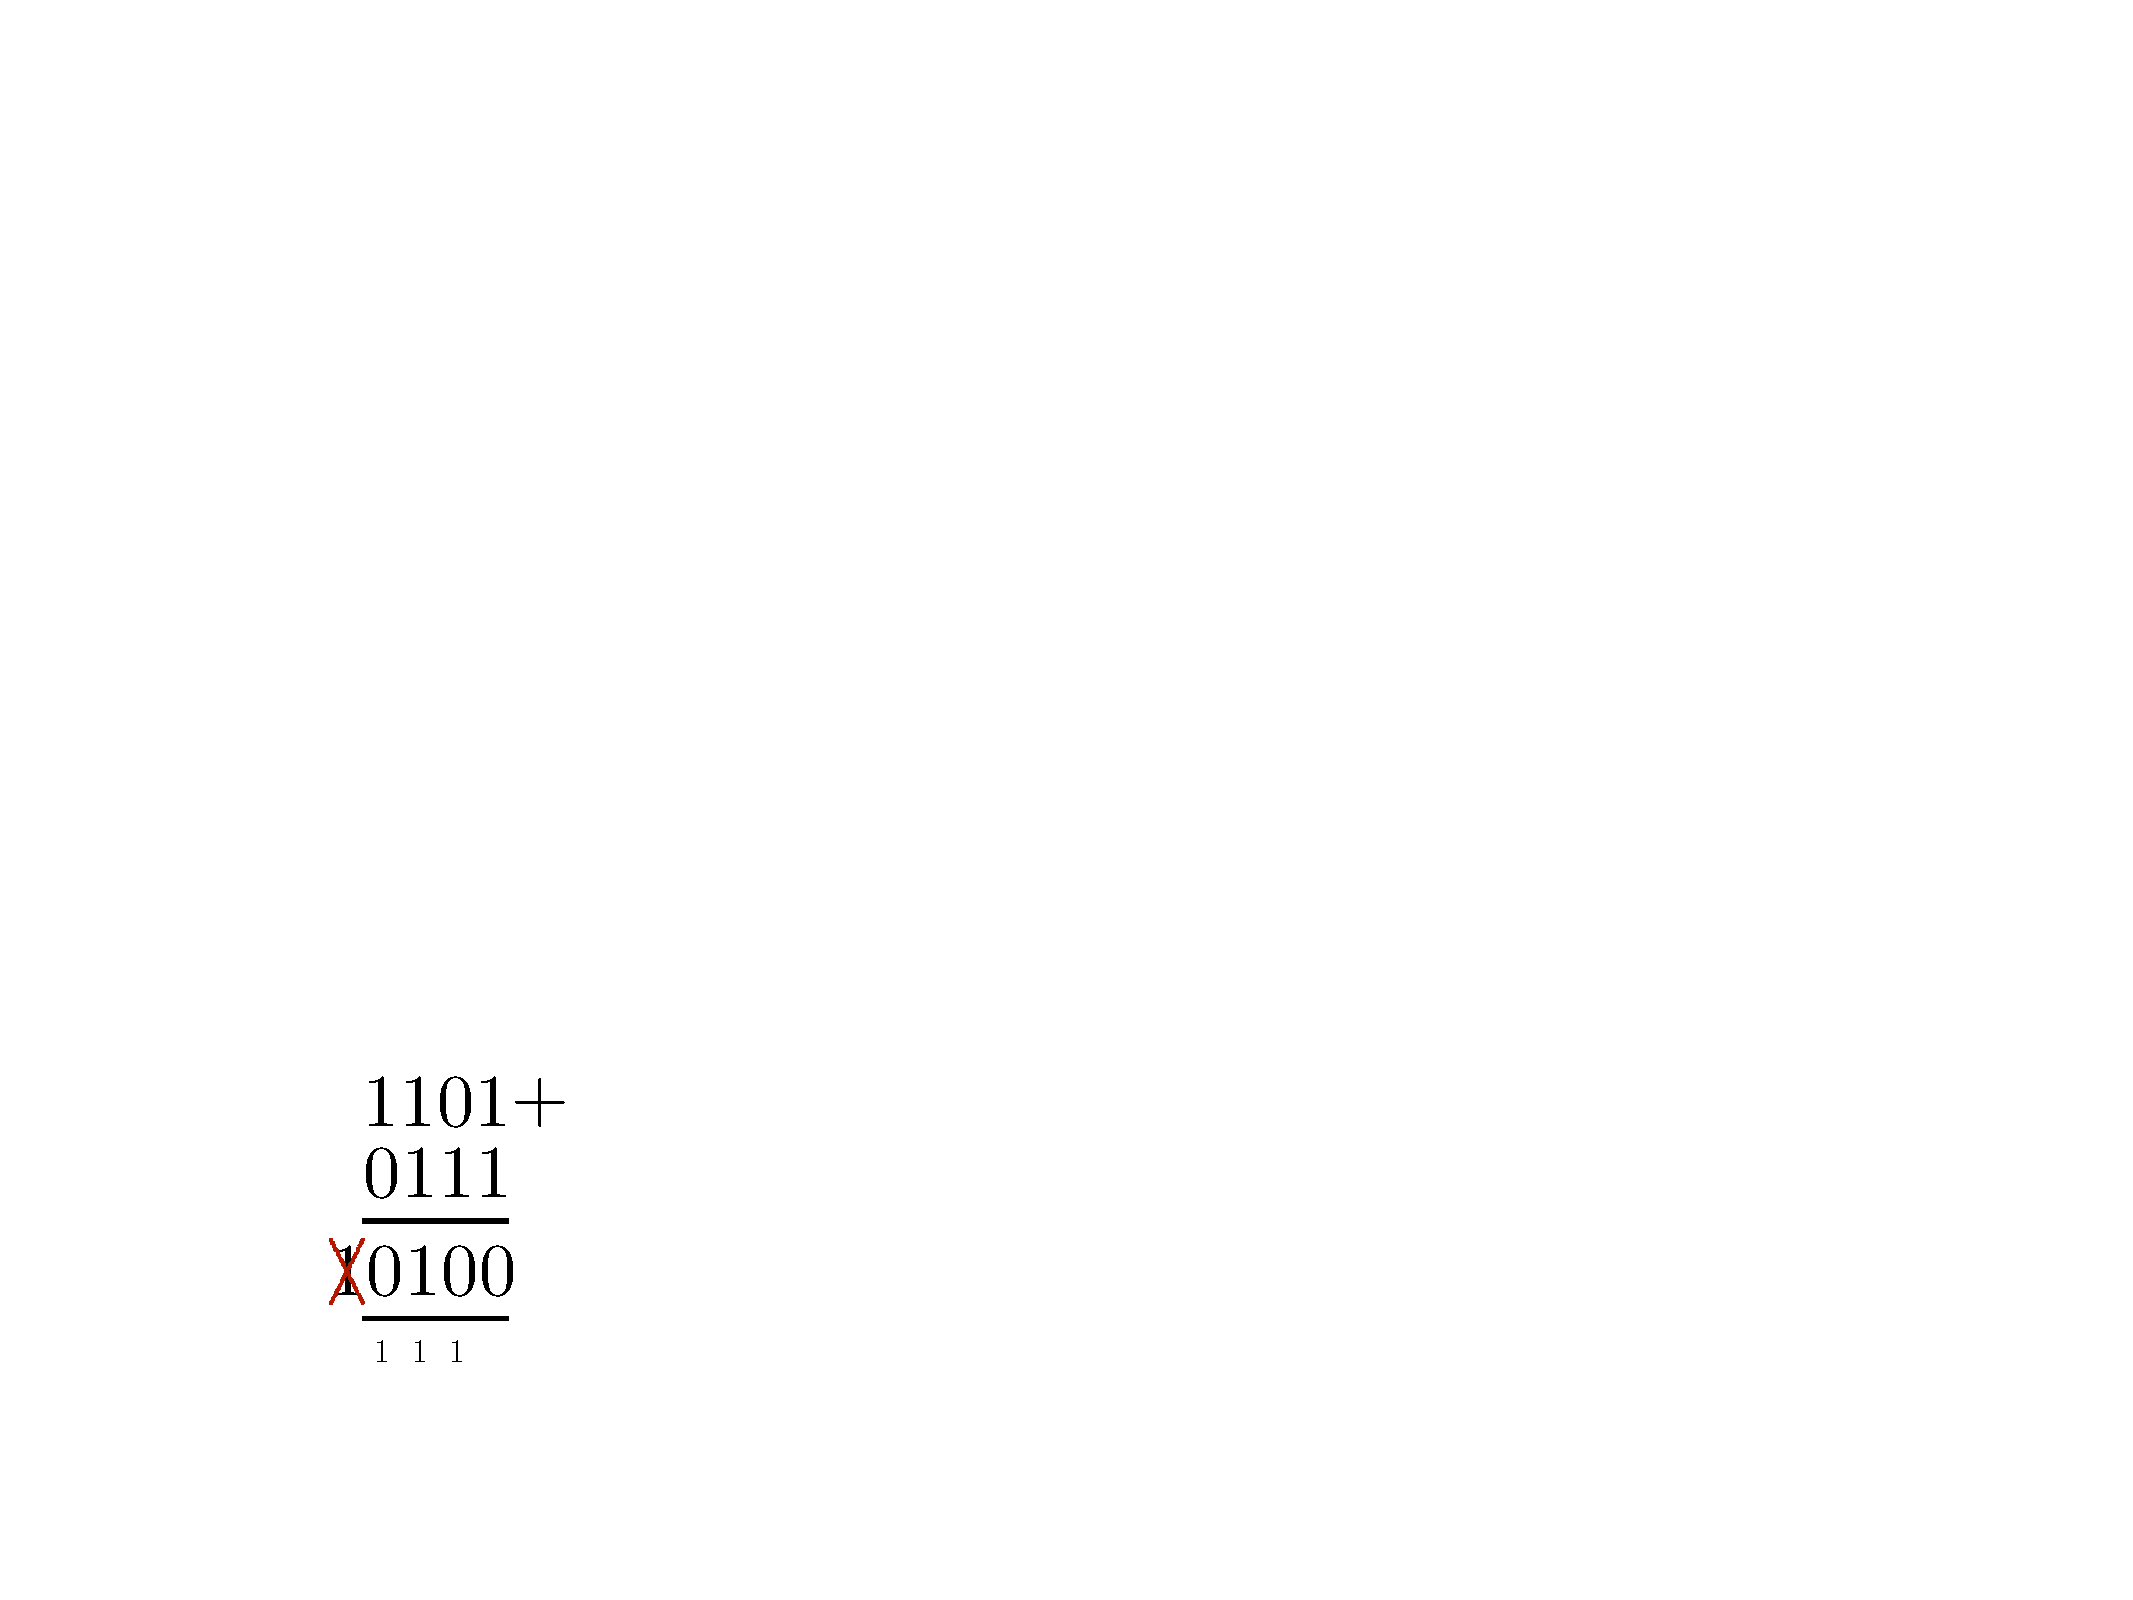
\includegraphics[width=0.1\textwidth]{figures/addition_example_2.pdf}
    \caption{Addition of $-3$ and $+7$ in binary}
    \label{fig:addition_example_2}
\end{figure}
For a final example of addition, let us consider $2-4$. We do this subtraction by considering it as $2+(-4)$, and then working out the twos complement representation of $-4$. To do this, start with $+4$, which is $B0100$, perform a bitwise not to obtain $B1011$, and add one LSB to obtain $B1100$. The addition is then carried out as shown in Figure \ref{fig:addition_example_3}. There turn out to be no carry bits necessary in this sum, and the resulting binary $B1110$ is $-2$ in decimal, as can be found out by subtracting $1$LSB to obtain $B1101$ and doing the bitwise not to obtain $B0010$, which is $+2$, hence the original $B1110$ must be $-2$. This is also confirmed by Table \ref{tab:twoscomplement}.
\begin{figure}[h!]
    \centering
    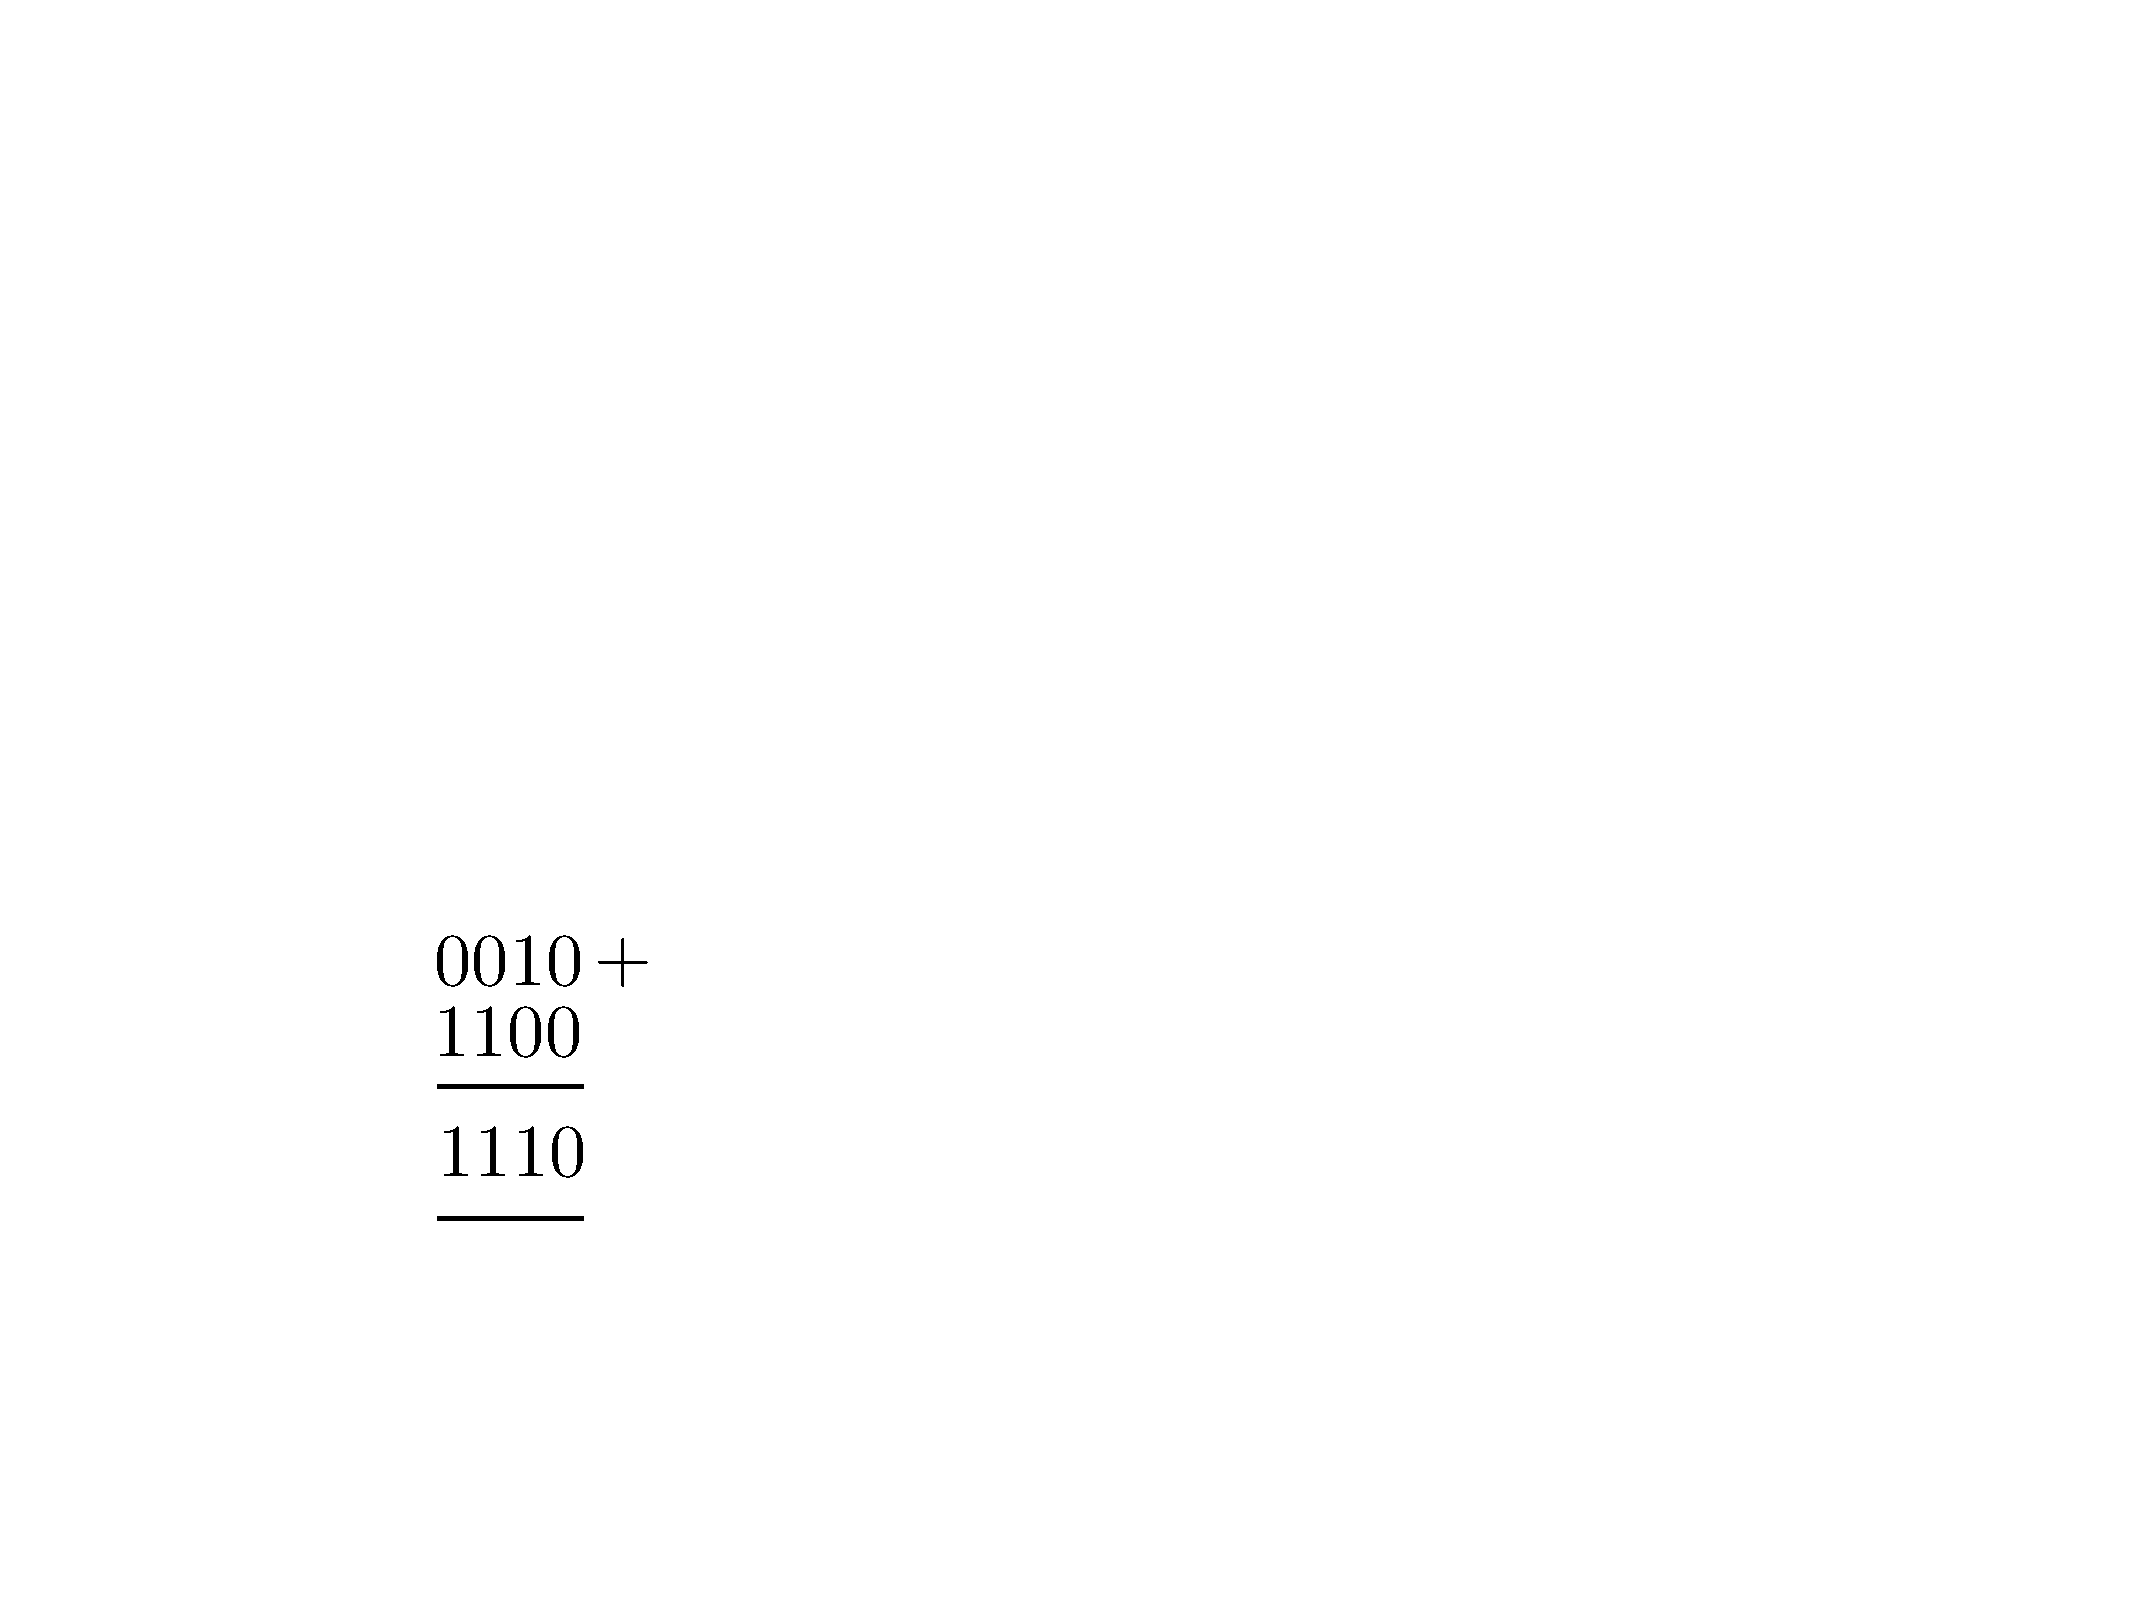
\includegraphics[width=0.1\textwidth]{figures/addition_example_3.pdf}
    \caption{The addition of $+2$ and $-4$.}
    \label{fig:addition_example_3}
\end{figure}

Next we move on to multiplication, which is carried out using the columnwise long multiplication technique you were taught in school. An example is shown in Figure \ref{fig:multiplication_example_1}.
\begin{figure}[h!]
    \centering
    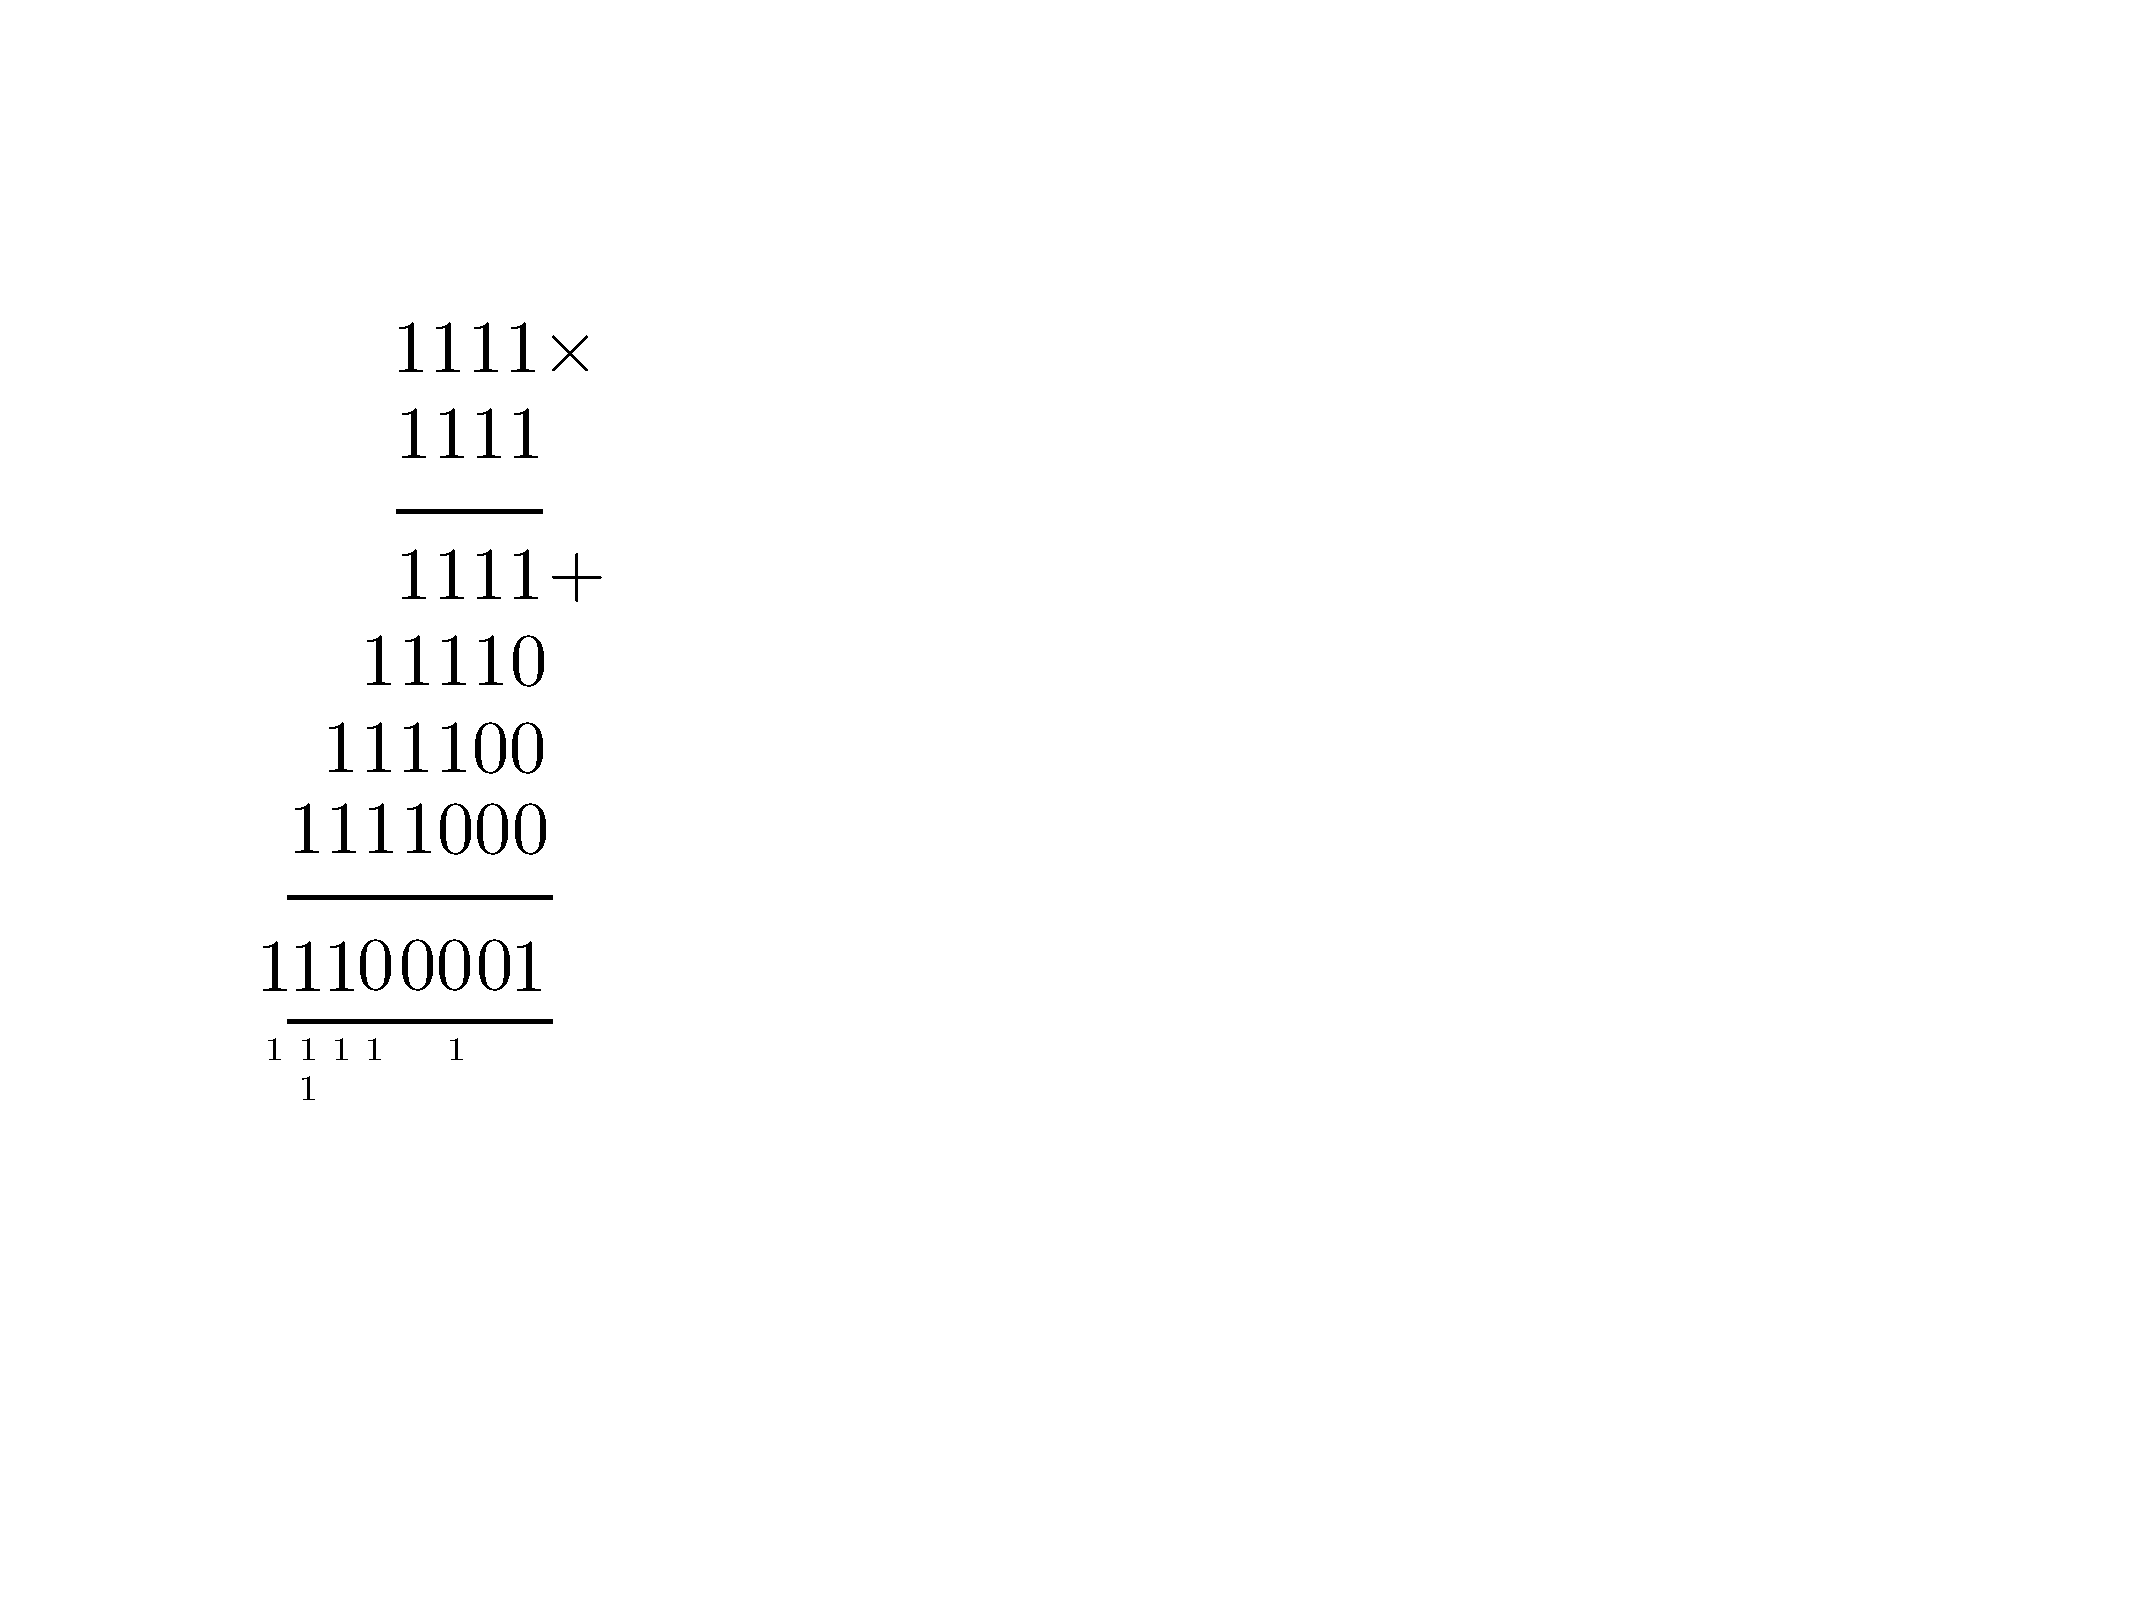
\includegraphics[width=0.18\textwidth]{figures/multiplication_example_1.pdf}
    \caption{Multiplication of the four bit representation of $-1$ by itself.}
    \label{fig:multiplication_example_1}
\end{figure}
The two inputs are $B1111$, which is the 4-bit twos complement representation of $-1$. We expect to obtain $-1\times-1=+1$. We proceed as we do in decimal long multiplication. First the least significant bit of the second number by all digits of the first one, placing the result on the top output row. Some notation if you haven't encountered it: a `leading' digit is one to the left of all the digits visible in a set of digits; a `trailing' digit is one to the right of those digits. Now add a trailing zero to the LSB of the next row, then proceed to multiply the second least significant bit of the second input number by the first row, and place the binary result to the left of the trailing zero. Repeat with the other two bits of the second input number. You will now have four rows containing binary numbers with one more bit in each successive row. Add the four rows up. 

When adding the four rows up we will encounter an oddity of addition that isn't often encountered in decimal column addition, although it can also happen. In the later columns, there end up being in some cases four or more $1$s to add. In these cases the result has more than two digits in binary. For example, in binary $B1+B1+B1+B1=B100$. In these cases you end up adding carry digits to other columns than that immediately to the left of the one you are working on. In the case of a $B100$ result in a column addition, you'd need to add a carry $1$ to the column two to the left of the current. And so on. In some cases there will end up being multiple carry $1$s in a column. This happens in in column 7 of the example. 

In fact, you only need to carry out sufficient columns of the multiplication and subsequent addition to get the result for the four least significant bits of the long multiply, because all higher bits are going to be discarded. The result, truncating to four bits, is $B0001$, so that in 4-bit twos complement binary $-1\times-1=+1$. So, everything seems consistent.

\section{Sign-extension}
\label{sec:signextension}

It often happens that you want to multiply two numbers represented
in some N-bit binary representation, and it is clear that the 
result is going to require more than N bits to represent it. 
When this happens, it is necessary to add more bits to the left
of the MSB in each of the input numbers. If you are using 
an unsigned representation, you just add zeros. However, if you
are in a twos complement signed representation, and the input 
number is negative, then the leftmost bit will be $1$. It turns
out that if you pad negative numbers, those with a leftmost $1$, 
with $1$'s to the left, then this maintains the binary number
as having the same numerical value in the expanded representation
with more bits, just as padding a positive binary number with 
zeros to the left maintains its value. This procedure of padding
based on the value of the most significant bit is called 
sign extension. The same rule applies to real numbers with 
fractional parts, which we discuss next.

\section{Fixed point arithmetic with real numbers}
\label{sec:fixedpoint}

Real numbers that are not integers, can be multiplied and added together using the same rules as described above, with three
additional new elements. The representation we arrive at 
after adding these elements is known as fixed point representation.
It is somewhat of a misnomer, because there is no
point in a binary sequence, and because the position of 
$2^0$ does in fact move around between columns as we shall
see. The terminology makes sense in the context of the 
popular floating point representation of numbers, where the 
position of the $2^0$ column is recorded in a second binary 
number, the exponent. Floating point numbers are in practice
tricky to manipulate digitally due to the large number of
special cases that are necessary to represent all the 
possible numbers in a range, so a discussion of them is beyond
the scope of this book. You can read about floating point
representation of numbers in \cite{Warren:10.5555/2462741}, 
chapter 17.

The first rule concerns how to represent the fractional 
portion of numbers. 
We are free to interpret any one of a sequence of bits
as representing the number $1=2^0$. When representing
integers, the rightmost bit
has been $1$, but if we were to make, say the third-rightmost
bit equal to $1=2^0$, then the bit to the right of it would 
be $2^{-1}=0.5$ and the LSB would be $2^{-2}$. In this 
representation, the smallest positive number that could be 
represented by the string of binary numbers would be $0.25$,
Let's say we have six bits in our number system, and let us 
say we wish to represent positive as well as negative real 
numbers. The largest positive number is represented by 
$011111$, which is $4+2+1+0.5+0.25=+7.75$. To find 
the representation of $-7.75$, do $\neg{B011111}+1{\rm LSB}$, 
which is $B100000+1{\rm LSB}=B100001$. The binary string for
$-0.25$ in this representation is $B111111$, since the smallest
negative number is all 1s. If we add this to the representation
of $-7.75=B100001$ and discard the overflow, we obtain
$B100000$, so the most negative number representable in six
bit twos-complement binary with $2^0$ represented by a 1
in the third-from-rightmost bit column is $-8$.

The second rule concerns how to work out the representation of
the answer. In addition, you ensure that the columns where
$1=2^0$ is written are the same in both inputs, and you follow
the same rule as for addition of signed integers, discarding any 
overflows in the result. For multiplication, you line up the
$2^0$ columns as before. In the result, the rule is that you
add the number of columns to the right of $2^0$ in the two 
inputs, and the sum of these numbers of columns is the number of
columns to the right of $2^0=1$ in the result. This exact same
rule is used to position the decimal point in 
the answer to the product of two decimal numbers.

\section{A fixed point multiplication example}
\label{sec:minusfourandaquarter}

Let us say we wanted to compute $-4.25^2$ in binary. In the
same 6-bit fixed point representation discussed in 
Section \ref{sec:fixedpoint}, $+4.25$ is $B010001$. We
find $-4.25$ by doing $\neg(B010001)+1{\rm LSB}$, which
is $B101110+1{\rm LSB}=B101111$. Next, we recognise that
we will probably need some more bits, so let's just
add another six bits to the right by sign extension,
so that we end up with a 12 bit representation of
$-4.25$, which is $B111111101111={\rm 0xfef}$. Not
wanting to do a tortuous long multiplication, I use
a web-based binary calculator to do the heavy lifting,
taking only the 12 least significant bits of the result, and I 
obtain $B000100100001={\rm 0x121}$.
Following the rule that you add the 
number of digits to the right of $1$ in each of the inputs,
there are $2+2=4$ digits to the right of 1 in this number,
so that the LSB represents $2^{-4}=0.0625$, which is 1/16.
The digits other two non-zero digits are 2 and 16, so the 
answer is $-4.25^2=16+2+0.0625=+18.0625$, which is correct.

\section{Summary of Chapter 1}
\label{sec:ch1summary}

In this chapter we have learned about the core logical operations
available on digital platforms, and how the fundamental operations
of arithmetic can be built up. We have learned how to represent
positive and negative real numbers using fixed point twos
complement representation. This will later on allow us to use
our digital platforms to do digital signal processing, which is 
one of the most important applications of digital signal processing
units. Hopefully you see how, in principle, complex numerical
calculations, at least those involving addition and multiplication
can be based on simple logical operations on strings of binary 
bits. You can now begin to appreciate what is inside a computer.
However, there are important fundamental elements still to introduce.
Fortunately, there are not that many more - in fact, we will meet
them both in Chapter \ref{sec:registers}.

\end{document}